%!TEX root = ../dissertation.tex

\begin{savequote}[75mm]
%%“Il Punto Interrogativo è il simbolo del Bene, così come quello Esclamativo è il simbolo del Male. Quando sulla strada vi imbattete nei Punti Interrogativi, nei sacerdoti del Dubbio positivo, allora andate sicuro che sono tutte brave persone, quasi sempre tolleranti, disponibili e democratiche. Quando invece incontrate i Punti Esclamativi, i paladini delle Grandi Certezze, i puri dalla Fede incrollabile, allora mettevi paura perché la Fede molto spesso si trasforma in violenza.”
%%Luciano De Crescenzo
%%“Prima di parlare domandati se ciò che dirai corrisponde a verità, se non provoca male a qualcuno, se è utile, ed infine se vale la pena turbare il silenzio per ciò che vuoi dire.”
%%Siddhartha Gautama
"Le parole sono atti, dei quali è necessario fronteggiare le conseguenze"
\qauthor{Gianrico Carofiglio}
\end{savequote}

\chapter{\textit{Hate Speech}}
\label{chap:hate}

\section{Libertà di parola o linguaggi d'odio?}
La riflessione sul discorso d’odio viene spesso ricondotta alla \textit{vexata quaestio} dei limiti della libertà di espressione. In particolare, negli Stati Uniti questo dibattito risulta molto spostato verso la garanzia del diritto di parola, sancito dal primo emendamento della costituzione che vieta esplicitamente al congresso di limitare la libera espressione di individui e stampa.

Proprio una ricercatrice statunitense, Katia Campbell, in un suo discorso del 2019 \citep{campbell2019}, spiega molto bene le origini di questo dibattito, in particolare nel mondo anglosassone. L'idea secondo cui la libertà di parola possa essere incondizionata si basa principalmente sulla teoria filosofica del "marketplace of ideas" che ha avuto un suo grande fautore nell'economista dell'ottocento John Stuart Mill \citep{mill1859}. A partire dalla corrente di pensiero liberista viene affermato come lo stato debba limitare il meno possibile gli individui (e il mercato), riconoscendo l'importanza del confronto dialettico, a partire dalla necessità di conoscere l'opinione opposta per poter essere realmente convinti della propria. Per evitare quindi la “tirannia della maggioranza” non si può proibire nessuna idea, neanche quelle ritenute scorrette o false dalla società stessa. Andando ancora più indietro nel tempo è possibile riscontrare nei sofisti greci le origini profonde di questo punto di vista. Per questi filosofi la natura della verità era infatti relativa e solo nello scontro tra argomenti diversi poteva nascere una vera democrazia. Per questo motivo i sofisti si sono dedicati all'insegnamento della retorica e della persuasione politica, ritenendoli strumenti indispensabili alla vita di ogni cittadin*, ancora più degli specifici valori morali.

In contrasto con questa teoria scettica, che arriva addirittura a domandarsi se la Conoscenza in quanto tale possa esistere, Campbell afferma come sia necessario porre dei limiti al linguaggio su basi etiche, affinché si possano salvaguardare tutte le componenti della popolazione che non hanno i mezzi per combattere ad armi pari all'interno dell'arena della società \citep{campbell2004}. Viene sottolineato come il linguaggio sia alla base della costruzione culturale, rimarcando la natura costituente della comunicazione. Utilizzando i fondamenti della "Critical Race Theory", Campbell afferma come sia necessario contestualizzare alcune delle norme presenti anche nella costituzione, affinché le leggi non diventino uno strumento per silenziare e marginalizzare le minoranze presenti nel paese. E’, inoltre,  importante creare un dibattito sano all'interno della società, che si basi anche sullo scontro di opinioni, ma  che escluda categoricamente menzogne o insulti. L'\textit{hate speech} viene descritto come dannoso su più livelli (individuale, comunitario e della società nel complesso) e una minaccia diretta all'equità necessaria a permettere la partecipazione di tutt* alla vita democratica.

Anche Popper prende una posizione molto netta nel dibattito sui limiti alla libertà di pensiero \citep{popper1945}. Con il suo "Paradosso della tolleranza", dimostra come sia necessario essere intolleranti con gli intolleranti, affinché si possa avere una società effettivamente tollerante. Nel libro “La società aperta e i suoi nemici” afferma che non è possibile assimilare la libertà di parola a discorsi discriminatori che vorrebbero mettere a tacere idee alternative. Un mondo in cui gli intolleranti possono promulgare i loro discorsi di odio in modo indisturbato rischia di diventare velocemente una società intollerante in cui, conseguentemente, la stessa libertà di parola risulta in pericolo. A partire da questo ragionamento, però, non si dice favorevole a limitare a priori la possibilità di espressione di tutte le persone definite come intolleranti. Piuttosto sostiene  che sia necessario mettere in campo meccanismi per combattere questo tipo di ragionamenti con argomentazioni razionali e, soprattutto, ritiene che sia indispensabile la massima vigilanza e partecipazione da parte dell'opinione pubblica sul tema. Queste strategie possono risultare molto più efficaci nel contrastare l'intolleranza della semplice censura generalizza. In casi estremi comunque, rivendica il diritto di poter sopprimere queste idee dannose, anche con la forza.

%[Fig.~\ref{hatefreespeech}]
\begin{figure}
	\centering
	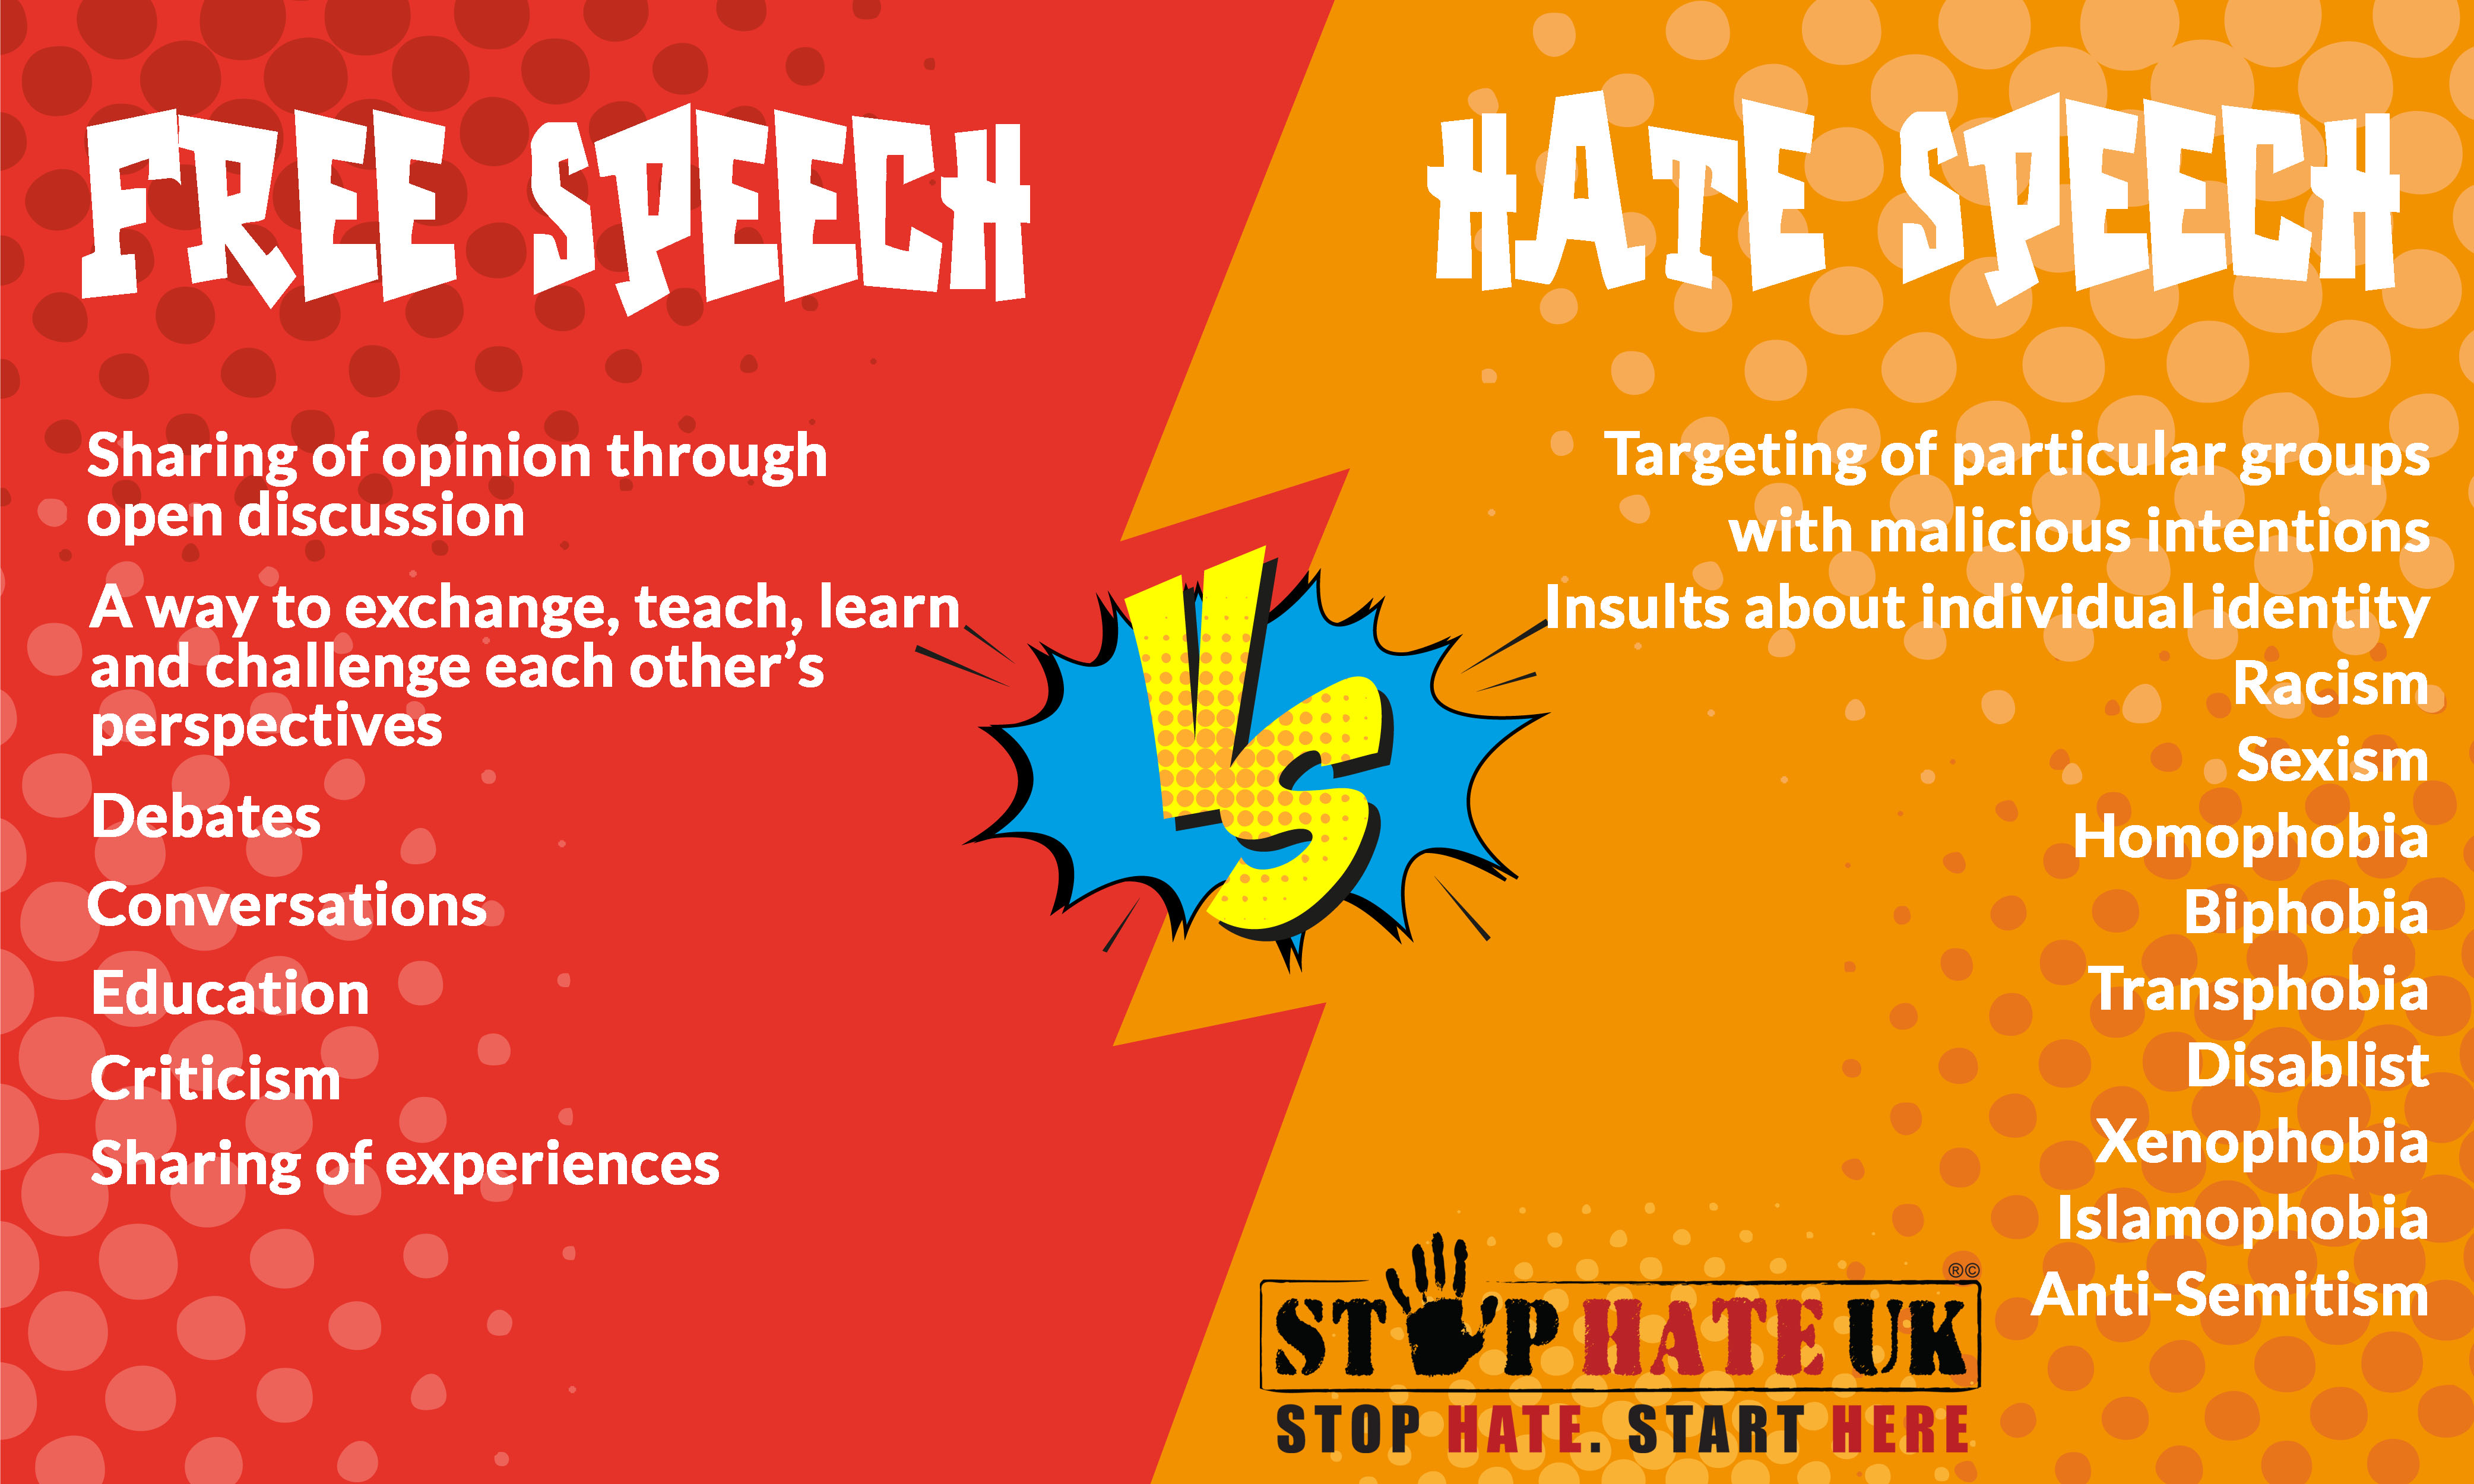
\includegraphics[width=0.7\textwidth]{figures/hatefreespeech}
	\caption{Rappresentazione schematica delle differenze tra libertà di parola e discorsi d'odio. Immagine pubblicata sul sito di Stop Hate UK.}
	\label{hatefreespeech}
\end{figure}

Un articolo in grado di sintetizzare e confrontare efficacemente tutte le posizioni emerse nel dibattito sui limiti alla libertà di pensiero è quello di Massaro \citep{massaro1990}. L'autore divide infatti le possibili interpretazioni dell'argomento in tre filoni principali: il primo tende a massimizzare le libertà individuali, proponendo di non punire l'\textit{hate speech} in nessun caso; al contrario il secondo punto di vista prevede l'utilizzo di tecniche di repressione del discorso d'odio per favorire la salvaguardia delle categorie maggiormente a rischio arrivando a ritenere punibile questo tipo di discorso in tutti i casi, non solo quando rivolto a settori della società e a categorie di persone definibili come vulnerabili; la terza opzione risulta una via di mezzo tra le prime due, prevedendo precise e progressive normative in grado di sanzionare solo gli attacchi basati su "razza, genere, religione, origini etniche, orientamento sessuale e altre caratteristiche protette". Il ricercatore si schiera in favore della terza via, in quanto in grado di recepire  i tratti positivi delle prime due e raggiungere una sintesi di compromesso. Questa è infatti la posizione condivisa, come vedremo, dalla maggior parte delle associazioni che si occupano del tema e dalle stesse piattaforme social.


\section{La definizione}
Anche la definizione di \textit{hate speech}, come quella di \textit{negative campaign},  risulta non univoca e differente a seconda dei contesti. Lo studio di Amnesty International, sulla base del quale è stata costruita la  presente ricerca, utilizza la definizione che viene data dalla Commissione Europea contro il razzismo e l'intolleranza nel 2015 \citep{ecri2015}:

\begin{displayquote}
	"[..] si intende per discorso dell’odio il fatto di fomentare, promuovere o incoraggiare, sotto qualsiasi forma, la denigrazione, l’odio o la diffamazione nei confronti di una persona o di un gruppo, nonché il fatto di sottoporre a soprusi, insulti, stereotipi negativi, stigmatizzazione o minacce una persona o un gruppo e la giustificazione di tutte queste forme o espressioni di odio testé citate, sulla base della "razza", del colore della pelle, dell’ascendenza, dell’origine nazionale o etnica, dell’età, dell’handicap, della lingua, della religione o delle convinzioni, del sesso, del genere, dell’identità di genere, dell’orientamento sessuale e di altre caratteristiche o stato personale."    
\end{displayquote}
Sempre nello stesso documento viene anche sottolineato che:
\begin{displayquote}
	"[..] il discorso dell’odio può assumere la forma di una pubblica negazione, banalizzazione, giustificazione o legittimazione dei crimini di genocidio, dei crimini contro l’umanità o dei crimini di guerra accertati dai tribunali, come pure di un’apologia delle persone condannate per avere commesso tali crimini"    
\end{displayquote}
Nell’accezione proposta dalla Commissione Europea, quindi,  l’odio non è riducibile ai semplici insulti generici, ha la particolarità di rivolgersi a una precisa minoranza già vittima di discriminazioni.

Uno studio pubblicato dall'UNESCO fornisce un quadro chiaro del contesto all’interno del quale si colloca la definizione di \textit{hate speech}, anche riguardo la sua versione online \citep{unesco2015}. Viene spiegato come quanto riportato nella Dichiarazione dei Diritti Umani (UDHR) all'interno della "International Covenant on Civil and Political Rights"(ICCPR) del 1966 \citep{iccpr1996} sia il vero fondamento della lotta all'odio, nonostante le trasformazioni della società e delle sue forme comunicative avvenute negli ultimi 60 anni.
In questo importante testo sui diritti politici e civili, all'articolo 19, viene sancita la libertà di parola, sottolineando però come sia necessario rispettare i diritti e la reputazione degli/delle altr*.
\begin{displayquote}
	\texttt{\textbf{Article 19}}
	
	"1. Everyone shall have the right to hold opinions without interference.
	
	2. Everyone shall have the right to freedom of expression; this right shall include freedom to seek, receive and impart information and ideas of all kinds, regardless of frontiers, either orally, in writing or in print, in the form of art, or through any other media of his choice.
	
	3. The exercise of the rights provided for in paragraph 2 of this article carries with it special duties and responsibilities. It may therefore be subject to certain restrictions, but these shall only be such as are provided by law and are necessary:
	(a) For respect of the rights or reputations of others;
	(b) For the protection of national security or of public order (ordre public), or of public health or morals."
\end{displayquote}
Nell'articolo 20, i limiti alla libertà di parola, già delineati nell’articolo 19, vengono ulteriormente specificati con l’affermazione che è necessario perseguire le discriminazioni razziali e religiose.
\begin{displayquote}
	\texttt{\textbf{Article 20}}
	
	"1. Any propaganda for war shall be prohibited by law.
	
	2. Any advocacy of national, racial or religious hatred that constitutes incitement to discrimination, hostility or violence shall be prohibited by law."
\end{displayquote}

I/le ricercat* che hanno partecipato allo studio UNESCO evidenziano che, benché esistano moltissime sfumature su base nazionale delle possibili definizioni di \textit{hate speech}, è necessario che tutte si conformino a questi principi generali, allargandoli il più possibile e non riducendone la capacità concreta di contrasto del fenomeno.

Viene inoltre sottolineano come sia importante anche per le piattaforme digitali raggiungere, oltre a una comune definizione di linguaggio d'odio, anche un accordo sulle iniziative da intraprendere per limitarne la diffusione.

Un passo in questo senso è stato fatto anche grazie alla campagna "Stop Hate for Profit" \citep{stophate2020}, già citata nel capitolo "\nameref{chap:introduzione}" della presente ricerca. Parallelamente a questa iniziativa, anche parte degli inserzionisti delle piattaforme social \citep{wfa2019} hanno deciso di affrontare l'argomento riuscendo a convergere su un'unica definizione di \textit{hate speech} fondamentalmente uguale a quella utilizzata nel presente studio. Nonostante ciò, rimangono ancora alcuni dubbi su quali iniziative concrete verranno prese dalle piattaforme nel breve periodo \citep{fischer2020}.

\vspace{5mm}

Allo stato attuale delle cose, analizzando i termini del servizio delle due piattaforme prese in considerazione in questo studio, possiamo trovare le seguenti informazioni.

\subsubsection{Twitter}
Twitter non menziona direttamente l'\textit{hate speech}, ma avverte i suoi utenti che "potrebbero essere esposti a contenuti che potrebbe essere offensivi", continua poi specificando che "in nessuna circostanza Twitter sarà responsabile in nessun modo di nessun contenuto" né dei relativi "danni per perdite di ogni tipo" che ne potrebbero conseguire. Nelle regole sulla pubblicazione di tweets viene aggiunto però che non è possibile "pubblicare o postare dirette, specifiche minacce o violenze contro altr*" \citep{twitter2019} e viene specificato come verrà applicata "tolleranza zero" a messaggi "violenti o discriminatori" sia nei tweet pubblici che nei \textit{Direct Messages}, pena "l'immediata e permanente sospensione dell'account".

\subsubsection{Facebook}
Facebook, invece, cita direttamente l'\textit{hate speech} definendolo come "gli attacchi diretti a persone sulla base di razza, etnicità, origini nazionali, credo religioso, orientamento sessuale, sesso, \textit{gender identity}, serie disabilità o malattie" e dichiarando la facoltà e la volontà di rimuoverlo dalla sua piattaforma  \citep{facebook2019}. Aggiunge poi che però "permetterà humour, satira sociale e commenti relativi a questi temi" ed invita gli/le utent* della piattaforma a utilizzare vere informazioni anagrafiche nel momento della registrazione, ritenendo che questo "aiuterebbe le persone ad essere più responsabili" e allo stesso tempo renderebbe  "le persone  sempre più consapevoli del tipo di \textit{audience} a cui si rivolgono" quando utilizzano la piattaforma. Viene quindi espressa una posizione molto precisa sull'anonimato come fattore in grado di aumentare il numero di contenuti d'odio, idea confermata anche dalla letteratura che affronteremo nei prossimi paragrafi.
%[Fig. ~\ref{facebookterms}]
%\begin{wrapfigure}{r}{5cm}
%    \fcolorbox{black}{yellow}{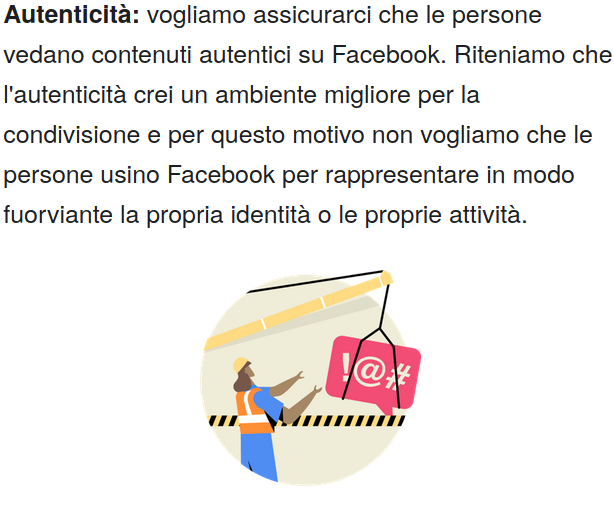
\includegraphics[width=5.5cm]{figures/facebookterms}}
%    \caption{Una delle specificazioni relative all'autenticità dei profili Facebook. Immagine contenuta all'interno degli standard della community di Facebook.}
%    \label{facebookterms}
%\end{wrapfigure}

\subsubsection{\textit{Dangerous Speech}}
Una ulteriore riflessione sul concetto di \textit{hate speech} viene invece proposta da Susan Benesch \citep{benesch2012}. Secondo l'autrice la definizione dei discorsi d'odio, anche in questo caso intesi come "discorsi che denigrano le persone sulla base dell'appartenenza a gruppi come quelli etnici o religiosi", risulta troppo ampia e non adatta a prevenire atrocità di massa per due ragioni: l'\textit{hate speech} è presente anche in nazioni in cui non vi è pericolo di genocidi; questo tipo di discorso non aumenta il rischio di crimini violenti di massa, anche se può arrecare seri danni emotivi e psicologici. L'obiettivo che si pone la ricercatrice keniota è quello di contestualizzare questa definizione per renderla più efficace in specifici contesti in cui i crimini d'odio sono molto frequenti ed estesi.
\begin{figure}
	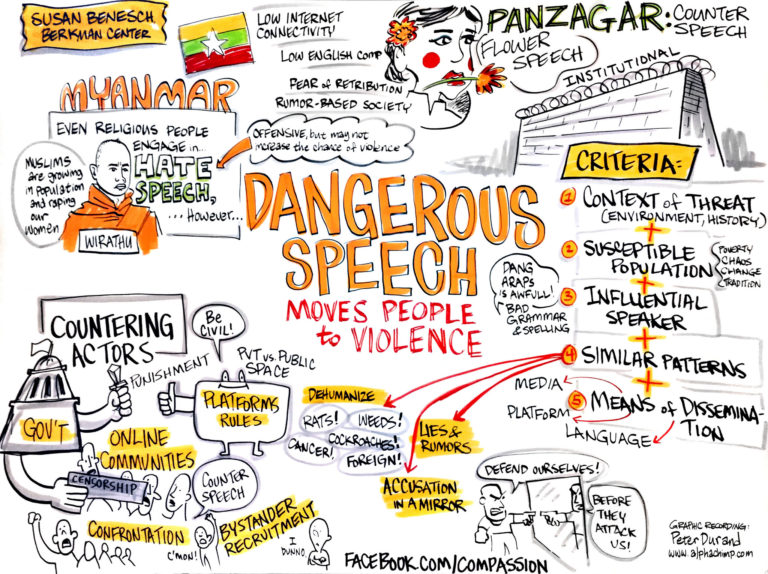
\includegraphics[width=\textwidth]{figures/dangerousspeech}
	\caption{Rappresentazione della definizione di Dangerous Speech realizzata da Peter Durand in seguito a una conferenza di Susan Benesch}
	\label{dangerousspeech}
\end{figure}

Viene quindi proposto il "\textit{dangerous speech}" inteso come discorso d'odio con una ragionevole probabilità di catalizzare o amplificare violenza di un gruppo verso un altro. La specificità di questa particolare accezione di \textit{hate speech} è quella di essere definita in base alle circostanze nelle quali viene propagandato [Fig.~\ref{dangerousspeech}]. Vengono infatti identificati alcuni fattori che, se presenti contemporaneamente, sono in grado di rendere più "pericoloso" un discorso d'odio: uno \textit{speaker} con un'altra influenza sul pubblico; un \textit{audience} con una paura latente che può essere coltivata da chi comunica; un discorso con un chiaro appello alla violenza; un contesto storico e sociale propizio alla violenza; la propagazione del discorso attraverso mezzi di comunicazione molto influenti, se non addirittura con il monopolio delle forti d'informazione disponibili.


\section{Discorsi d'odio e crimini d'odio}
Il primo caso conclamato di effetti estremamente negativi nella vita offline a seguito di campagne di odio diffuse attraverso canali di comunicazione digitali è quello delle elezioni in Kenya del 2007 \citep{osborn2008}. In seguito a quella tornata elettorale si generò un’ondata di violenza che portò all'uccisione di più di mille persone, altre 600mila furono sfollate. In quell'occasione le \textit{Information Communication Technologies} hanno svolto per la prima volta un ruolo fondamentale nel contesto elettorale. Come suggerito da Osborn infatti, tramite SMS, e-mail e siti web, sono state diffuse una serie di notizie false e incitazioni all'odio che hanno determinato un contesto sociale estremamente instabile e pericoloso. Attraverso un grande numero di interviste e osservazioni partecipate, l'autore è riuscito a ricostruire l'origine e la forma di diffusione di questi contenuti, ottenendo una significativa mappa degli effetti che ne sono susseguiti, nonostante questo fosse uno tra i primi studi del suo genere.

Durante le successivi elezioni Keniote del 2013, è stato condotto uno studio molto più ampio e sistematico dei canali di comunicazione digitale e delle conseguenze che ne sono scaturite. Utilizzando la definizione già citata di \textit{dangerous speech} elaborata da Susan Benesch \citep{benesch2012}, sono stati  raccolti per sei mesi tutti gli episodi di \textit{hate speech} tramite interviste, monitoraggio di siti online e una raccolta di messaggi ricevuti da singoli individui, sia in inglese che nei dialetti locali. Successivamente sono stati codificati i contenuti selezionati in base a due livelli di odio: \textit{hate speech} o \textit{dangerous speech}. Benché all'epoca solo il 35\% della popolazione locale avesse accesso ad internet e solo metà di queste persone avesse un profilo Facebook, nonostante quindi la parte di popolazione presente su questo social network fosse quella più giovane e urbanizzata, quindi la meno incline all'odio razziale, è stato riscontrato che ben un contenuto d'odio su quattro era assimilabile al \textit{dangerous speech} in quanto conteneva incitazioni dirette all'uccisione di membri della fazione rivale. Interessante notare che molti degli utenti protagonisti di questi attacchi, a poca distanza dalle esternazioni avevano cambiato nome del profilo, dando un'ulteriore conferma della teoria (che vedremo tra poco) dell'anonimato come disinibitore di atteggiamenti aggressivi online. Altro dato, particolarmente interessante per alla presente ricerca, riguarda i canali su cui l'odio si è propagato durante il periodo di monitoraggio: solo il 3\% del totale è stato riscontrato su Twitter, mentre oltre il 90\% ha avuto luogo su Facebook. Secondo gli/le ricercator*, questo potrebbe essere dovuto alle caratteristiche della piattaforma di Mark Zuckemberg nella quale è possibile discutere anche in gruppi e pagine specifiche e non solo in trend pubblici come su Twitter, dando la possibilità di comportarsi in modo diverso in base all'ambiente con il quale si interagisce. Quest'ultimo dato è però legato anche all'utilizzo particolare dei social media da parte della popolazione Keniota, rimane quindi un dato difficilmente generalizzabile ad altre nazioni e periodi storici.

La relazione con l'\textit{hate speech} online è stata indagata anche in nazioni in cui l'\textit{hate crime} non si configura come un fenomeno di massa. Come dimostrato da uno studio condotto nel 2019 a Londra tramite l'utilizzo di tecniche di \textit{Computational Criminology} \citep{williams2019}, è possibile riscontrare un'associazione tra i discorsi d'odio riguardo razza e religione registrati su Twitter e crimini d'odio aggravati da discriminazioni dello stesso tipo avvenuti in un determinato luogo. Per questa ricerca sono stati confrontati, in un periodo di otto mesi, i dati della polizia anticrimine e quelli dei social di microblogging, trovando una relazione spaziale e temporale tra i due tipi di fenomeno. Come possiamo osservare nella figura \ref{fig:hatetweet}, la correlazione tra le due serie di dati risulta significativa (l'intervallo di confidenza al 95\% è rappresentato in grigio).
\begin{figure}
	\centering
	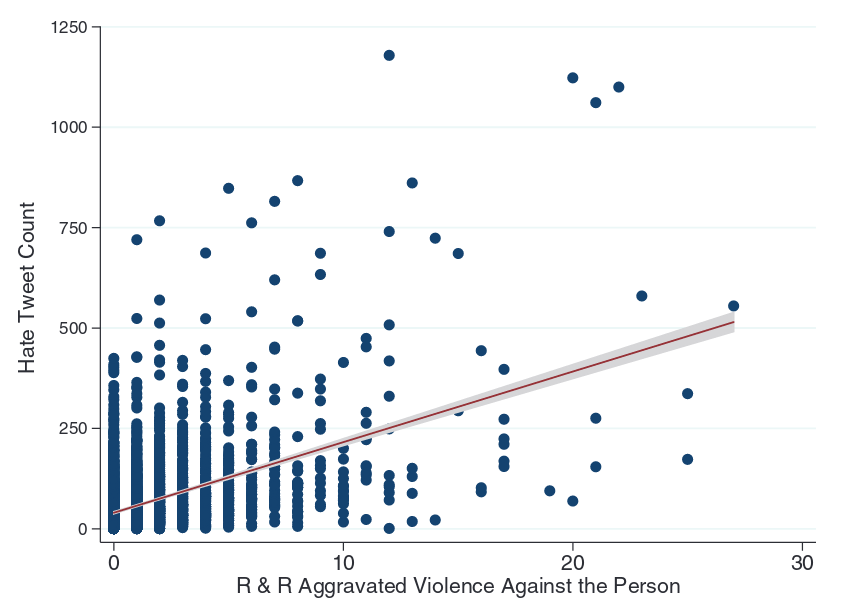
\includegraphics[width=0.7\textwidth]{figures/hatetweet}
	\caption{La correlazione tra il numero di tweet di odio e il numero di crimini d'odio. Immagine pubblicata nello studio di Williams (2019).}
	\label{fig:hatetweet}
\end{figure}

Anche in uno studio analogo svolto in Germania, in cui sono state analizzate le discriminazioni rivolte ai rifugiati, le conclusioni sono le stesse: il sentimento anti-rifugiati rilevato su Facebook predice il numero di crimini d'odio legati a questa categoria di persone  \citep{muller2019}. Nello studio viene preso in considerazione il partito “Alternative f̈ur Deutschland” (Alternativa per la Germania, AfD), fazione di estrema destra con posizioni fortemente anti-rifugiati diventata il terzo partito nelle elezioni federali del 2017. Qui viene analizzata la loro pagina Facebook poiché in grado di far registrare un numero di interazioni molto alto e nettamente superiore agli altri due principali partiti tedeschi (300mila followers e 175mila posts nel 2017). La particolarità di questa pagina è quella di lasciar pubblicare a qualsiasi utente direttamente sulla propria bacheca, non moderando in nessun modo i messaggi di odio che vi vengono generati. L’esito di questa strategia è  una percentuale di post relativi alla questione rifugiati molto maggiore rispetto ai media tradizionali e con molti messaggi identificati come \textit{hate speech}. I ricercatori hanno incrociato  i dati provenienti da  questa pagina con quelli di varie associazioni ed istituzioni che monitorano i crimini d'odio, giungendo a un database complessivo che ha coperto  4 466 municipalità tedesche in un periodo di più di due anni, tra il 2015 e il 2017. Tramite le API di Facebook sono stati  estratti 176 153 posts, 290 854 commenti, 510 268 likes, e 93 806 user ID individuali dalla pagina dell' AfD. Le analisi confermano l’esistenza di una significativa correlazione tra i due fenomeni, soprattutto in presenza di avvenimenti particolarmente salienti per l'opinione pubblica, come possiamo vedere nel grafico riportato [Fig. \ref{fig:afd}].
\begin{figure}
	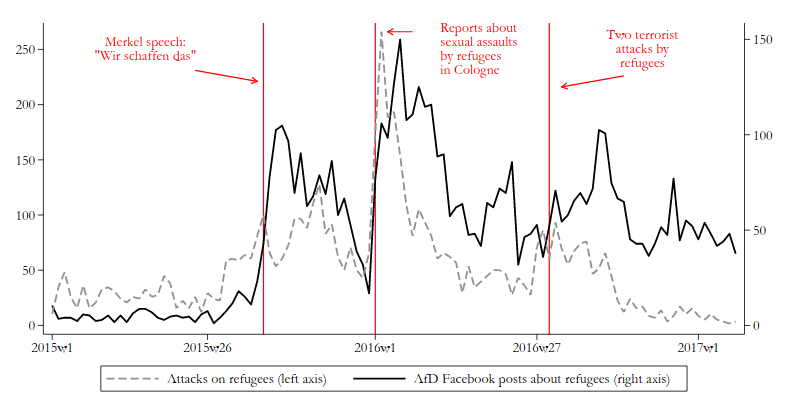
\includegraphics[width=\textwidth]{figures/afd}
	\caption{Il numero di post anti-rifugiati sulla pagina Facebook dell'Afd e il numero di crimini anti-rifugiati in Germania, nel corso del tempo. Immagine pubblicata nello studio di Muller e Schwarz (2019).}
	\label{fig:afd}
\end{figure}

\section{Discorsi d'odio online}
Se è stata accertata una relazione tra odio online e crimini di odio offline, diventa rilevante una riflessione sulle specificità dell’\textit{hate speech} generato sul web rispetto a quello presente nei media tradizionali. Di questo si occupa uno studio di Brown \citep{brown2018}. Lo studioso inizia riprendendo le caratteristiche proprie dell’odio online, definito anche come "cyberhate", già presenti in letteratura: la facilità di accesso allo strumento, la dimensione dell'\textit{audience} facilmente raggiungibile e la possibilità di restare anonimi (tratteremo quest'ultimo aspetto in modo approfondito più avanti). Per sintetizzare e specificare meglio accessibilità e potenza della comunicazione digitale, Brown propone un quarto aspetto che chiama "istantaneità", facendo riferimento alla estrema velocità con la quale è possibile pubblicare contenuti su internet, rendendo più spontaneo e più sconsiderato il linguaggio di chi comunica. Tramite l'esempio dell'ipotetica diffusione di un messaggio antisemita, confrontato il tempo richiesto per raggiungere la stessa \textit{audience} con un tradizionale volantinaggio rispetto alla pubblicazione di un contenuto sui social media, appare chiaro quanto i tempi vengano ridotti da ore (se non giorni) a solo alcuni \textit{istanti}, appunto.
Viene sottolineato inoltre che non ci sono particolari differenze di sostanza negli attacchi d'odio tra online e offline, quello che risulta sicuramente diverso è il modo in cui questo linguaggio viene moderato (o meglio non moderato) su piattaforme digitali rispetto a media tradizionali e vita offline. Sulle principali piattaforme digitali non vengono infatti imposte le stesse restrizioni adottate dalle \textit{media companies} tradizionali come, ad esempio, le linee editoriali o i codici di condotta. Inoltre, il carattere di “istantanietà” dei messaggi online permette la pubblicazione di messaggi scritti istintivamente, senza alcuna riflessione
e prima che si possano attivare freni inibitori. Tutto questo favorisce la diffusione dell’odio.

\subsubsection{Strumenti di crowdsourcing per combattere l'odio}
Se da una parte lo sviluppo dei social media ha dato luogo a un nuovo tipo di modalità di propagazione dell'odio, ha anche dato la possibilità di ripensare gli strumenti con i quali è possibile combatterlo.
Esistono almeno due associazioni che nel mondo si occupano di creare mobilitazioni tra gli utenti di internet tramite \textit{crowdsourcing} di contributi indirizzati a catalogare e studiare i contenuti di odio online. Il loro obiettivo pratico è quello di costruire strumenti innovativi in grado di tracciare l'\textit{hate speech} sui social network contribuendo a migliorare le policy delle varie piattaforme e a contrastare i fenomeni d'odio in generale.
Una di queste è HateBase (\thefootnote{\url{hatebase.org}}) e si occupa di censire e localizzare  i discorsi d'odio su internet per costruire una mappa degli attacchi e della loro propagazione. Un fondamentale contributo di questa associazione è la creazione (e l'aggiornamento costante) di un dizionario con le specifiche parole d'odio usate in tutto il mondo, a seconda delle particolarità che il lessico assume nelle varie nazioni e lingue. La realizzazione di questo strumento è stata possibile grazie alla collaborazione di migliaia di persone che hanno aiutato a verificare esempi di discorsi d'odio, confermandone la natura in una specifica comunità.

The Online Hate Prevention Institute (\thefootnote{\url{ohpi.org.au}}), invece, combatte l'odio con un applicazione web che consente a tutti gli utenti di internet di segnalare l’\textit{hate speech} pubblicato sui vari social network. La possibilità di tenere traccia delle segnalazioni, che poi vengono inoltrate alle stesse piattaforme, permette di registrare i tempi di reazione di queste ultime e la loro celerità nel rimuovere i contenuti incriminati.

\section{Discorsi d'odio e caratteristiche personali}
Oltre agli aspetti in grado di aumentare la diffusione dell'odio generati dalle proprietà del mezzo di comunicazione come la già citata istantanietà, sono presenti in letteratura anche studi che considerano le caratteristiche soggettive di chi diffonde l'odio. Forse la più significativa è l'anonimato. In uno studio del 2004 \citep{suler2004}, viene preso in considerazione "l'effetto disinibizione" presente nel mondo online a partire dall'assunto che gli episodi di \textit{self-disclosure} sono più frequenti nelle interazioni nel cyberspazio rispetto a quelle di persona. Se da una parte la comunicazione digitale porta con sé una "disinibizione benigna" in grado di spingere a condividere parti molto personali della propria vita, dall'altra parte può portare anche a una "disinibizione tossica" quando i soggetti si ritrovano ad usare un linguaggio incivile che altrimenti non userebbero o quando si trovano ad esplorare ambienti online legati a criminalità, violenza o pornografia che non frequenterebbero mai nella vita offline. Benché la distinzione tra questi due tipi di disinibizione online possa risultare per alcuni aspetti controversa poichè basata su cosiderazioni di valore, l'articolo di Suler cerca di individuare le cause alla base del fenomeno indipendentemente dai suoi risvolti positivi o negativi. Vengono individuati sei principali fattori alla base della disinibizione online riassunti nella seguente tabella:

\setlength{\arrayrulewidth}{0.8mm}
%\setlength{\tabcolsep}{28pt}
%\renewcommand{\arraystretch}{1.5}
\newcolumntype{P}[1]{>{\centering\arraybackslash}p{#1}}

\begin{tabular}{|P{0.2\textwidth}|P{0.7\textwidth}|  }
	\hline
	\multicolumn{2}{|c|}{\texttt{\textbf{\textcolor{SchoolColor}{I sei fattori della disinibizione online secondo Surel (2004)}}}} \\
	\hline
	\texttt{\textbf{Nome del fattore}} & \texttt{\textbf{Descrizione del fattore}}\\
	\hline
	Anonimato dissociativo   & Deriva dall'utilizzo di un profilo falso o animo che rende meno vulnerabili alle conseguenze di un comportamento, dissociando l'identità online da quella offline.\\
	\hline
	Invisibilità & A causata dall'impossibilità di vedere chi sta frequentando un determinato ambiente digitale come un sito internet, l'invisibilità può generare una propensione a visitare luoghi (digitali) dove altrimenti non si andrebbe se si fosse visti. Eliminare il linguaggio del corpo ed espressioni facciali in grado di far trasparire, per esempio, la disapprovazione o la noia, riduce le inibizioni.\\
	\hline
	Asincronia & L'asincronia della comunicazione digitale rende possibili interazioni "mordi e fuggi" in cui si rispondere a messaggi e subito ci si disinteressa della risposta, per poi leggerla quando si è nello stato emotivo migliore per accettarne le conseguenze.\\
	\hline
	Introversione solipsistica & Comunicazioni solo testuali possono indurre chi comunica a immaginare la voce e il volto della persone con cui si sta parlando, trasformando una figura digitale in un personaggio intra-psichico. Questo può portare a pensare discussioni online come se fossero all'interno della propria mente, aumentando la disinibizione.  \\
	\hline
	Immaginazione dissociativa & È possibile che relazioni sviluppate nel cyberspazio diano luogo alla una netta separazione tra le regole e i comportamenti adottati online rispetto a quelli offline, delineando una separazione tra due mondo che in realtà non sono del tutto separati e spingendo ad aumentare la disinibizione dei comportamenti violenti.\\
	\hline
	Minimizzazione di status e autorità    &  Negli ambienti digitali molti dei simboli di status e potere presenti nelle relazioni dal vivo vengono meno, diminuendo la paura di disapprovazione e punizioni che ne deriva e facilitando una maggiore disinibizione\\
	\hline
\end{tabular}

Nello studio viene inoltre sottolineato come anche le differenze individuali possano giocare un ruolo in questo fenomeno. Differenti personalità mettono in campo diversi meccanismi di difesa in grado di regolare la disinibizione. Ad esempio, personalità istrioniche tendono ad essere più aperte e disinibite, mentre persone compulsive possono mostrare tendenze opposte.
In ogni caso, la presenza dei sei fattori alla base della disinibizione individuati da Surel favorisce l’esternazione di messaggi di odio online.

%da yacubov2020 -->
%studies find that uncivil discourse is a per-vasive  feature  of  online  political  talk,  and  it  is  facilitated  by  several affordances of computer-mediated  communication,  such  as  anonymity  and  the  possibility  to  engage with unknown others, as well as greater likelihood to be exposed to disagreeable per-spectives [2, 3]
%2 Papacharissi,  Z.:  Democracy  online:  civility,  politeness,  and  the  democratic  potential  of online political discussion groups. New Media  Society. 6, 259–283 (2004).


%---> \citep{mondal2017}the effect of anonymity on hate speech and the most hated groups across regions. In order to achieve our objectives, we gather traces from two social media systems: Whisper and Twitter


Un altro studio più recente ha indagato in laboratorio come le interazioni intergruppo possano incidere sulla percezione dei commenti di odio online \citep{kim2018}. In questo articolo i commenti online sono stati classificati come contatto intergruppo diretto (quando viene nominato esplicitamente un membro dell'outgroup) o come contatto intergruppo indiretto (quando si legge un commento di un membro dell'outgroup non diretto a sé stessi). In particolare sono state  prese in considerazione le reazioni ad articoli di giornali, considerati un luogo di scambio di opinioni, anche opposte, molto utilizzato nell'ultimo decennio. Il modello testato utilizzava le emozioni negative e positive come mediatori degli effetti dei contatti tra gruppi e come output il livello di minaccia ("generale", "simbolica" e "realistica") e la distanza sociale. Sono stati,  quindi, selezionati 397 partecipanti dell'esperimento tutt* contrar* all'avanzamento dei diritti su due temi, quello dell'omosessualità e quello dell’ immigrazione. Sono stati presentati loro alcuni articoli di giornali e i relativi commenti in due situazioni sperimentali: con contatto indiretto o diretto.

Dai risultati emerge che nel caso del tema omosessualità il contatto diretto influisce positivamente sulla riduzione della minaccia generale e simbolica, e sulla distanza sociale, ma non sembra avere effetti sulla percezione di minaccia realistica. Nessuno di questi indicatori è invece significativamente modificato nel caso del tema immigrazione. I test sul contatto indiretto, invece, non hanno registrato nessuna variazione significativa negli indicatori considerati come output.
Inoltre, considerando le emozioni positive provate durante la lettura dei commenti come mediatore del tipo di contatto, si registrano aumenti significativi nella riduzione di tutti i tipi di minaccia e di distanza sociale, sia in relazione all’omosessualità che all’immigrazione, ma sempre solo in presenza di contatti diretti. Le emozioni negative diminuiscono alla lettura di commenti riguardanti l'omosessualità, e risultano mediatori nella riduzione di tutti i tipi di minaccia e la distanza sociale, ma non producono effetti significati quando il tema è 'immigrazione.
Nonostante il fatto che a volte le interazioni online siano utilizzati per diffondere odio e quindi aumentare la diffusione di stereotipi, possiamo concludere affermando che i contatti online positivi con membri dell'outgroup, sopratutto se diretti e non estesi, possono anche aiutare a ridurre il pregiudizio.

Anche gli orari in cui l'odio online viene prodotto ci possono fornire degli importanti spunti per capire che tipo di persone mettono in pratica questi comportamenti.
Come riportato da un'altro studio di un'associazione inglese \citep{cts2019}, dalle ricerche effettuate su Google è possibile trarre alcune interessanti considerazioni. In questo caso specifico sono state analizzate le ricerche che utilizzano un linguaggio o dei contenuti discriminatori nei confronti della comunità ebraica sul più famoso motore di ricerca. Sono state trovate 170mila ricerche di questo tipo in un anno in Inghilterra, nazione che si posiziona, così, al terzo posto nel mondo per ricerche sul’antisemitismo, dietro solo a Israele e Libano, con percentuali 29 volte superiori, ad esempio a quelle degli Stati Uniti. Come possiamo osservare dal grafico riportato nello studio, il 10\% delle ricerche contiene "pensieri violenti", dovuti alla presenza di frasi come "Gli ebrei devono morire" o "Uccidere gli ebrei" [Fig. ~\ref{google}]. Interessante come la maggior parte di queste ricerche sia stata effettuata tra le 2 e le 3 del mattino. In questo momento della giornata sono concentrate in generale la stragrande maggioranza delle ricerche che fanno riferimento a comportamenti omicidi, ma anche suicidi, dimostrando come istinti violenti contro sé e contro gli altri abbiano una radice comune, da ricercare nella personalità e negli stati emotivi dei soggetti interessati.

\begin{wrapfigure}{r}{7cm}
	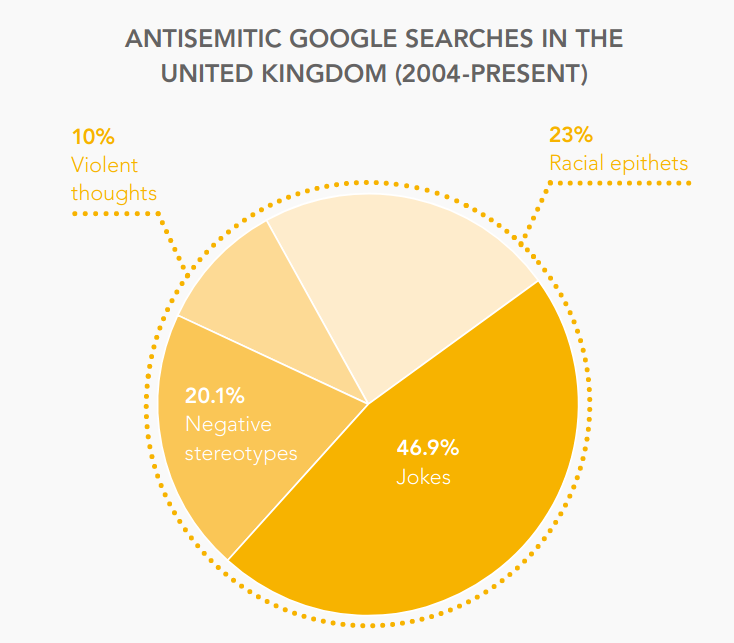
\includegraphics[width=\linewidth]{figures/google}
	\caption{Percentuali di tipo di odio registrato nelle ricerche effettuate su Google in Inghilterra. Immagine pubblicata nello studio del CTS (2019).}
	\label{google}
\end{wrapfigure}

Un altro articolo ha invece indagato le caratteristiche della personalità di chi odia online \citep{erjavec2012}.In questo caso l'ambito di ricerca non ha riguardato i social network, ma i commenti agli articoli giornalistici pubblicati sui tre principali siti web di tre testate giornalistiche slovene. A differenza di altre ricerche, oltre all'analisi del discorso applicata ai contenuti online che compongono il campione di riferimento, sono state  eseguite approfondite interviste con chi ha prodotto i contenuti, al fine di indagare le caratteristiche di chi diffonde odio. In seguito a tali interviste è stata fatta una classificazione dei soggetti coinvolti su un continuum che va dalla personalità autoritaria  a quella libertaria sulla base di tre dimensioni principali: la relazione con la società; la dimensione cognitiva ed intellettuale; la relazione con gli altri. All'estremo dell’autoritarismo possiamo trovare, ad esempio, individui con grande rispetto per le autorità, tendenze al pregiudizio e fedeltà incondizionata verso il proprio gruppo di appartenenza. All'altro estremo si collocano persone con vocazione alla libertà ed all'equità, anticonformiste e tolleranti, più indipendenti dal gruppo di riferimento e indirizzate alla realizzazione personale.
Sulla base di queste interviste sono stati definiti due diversi  profili degli odiatori: da una parte quelli che sono organizzati e fanno riferimento a un particolare gruppo politico e ai suoi interessi, dall'altra quelli che agiscono in autonomia. Gli appartenenti al primo gruppo vengono definiti "i soldati" poiché appartengono a partiti o organizzazioni non governative, utilizzano discorsi militari, rispondendo a ordini dei loro superiori, e agiscono nell'ottica di completare le missioni assegnate difendendo i loro interessi e cercando di "distruggere il nemico". Nel secondo gruppo vengono inseriti i "believers", i "players" e i "watchdogs". I primi seguono la loro ideologia personale e le loro regole nell'ottica di attaccare il nemico, spesso utilizzano pseudonimi con significati precisi che richiamano alla giustizia e la leadership, assumendo il ruolo degli unici a dare la giusta interpretazione delle notizie, giustificando i loro attacchi di odio come l'unica modalità possibile per affermare la verità. Il secondo sottogruppo usa l'\textit{hate speech} come un'arma in un gioco all'interno di una comunità digitale, dimostrando di non avere una particolare visione politica, ma di usare vari punti di vista in modo strumentale. Questo gruppo vede gli attacchi non come veri discorsi d'odio, ma come scherzi. L'ultimo profilo delinea un gruppo di persone che postano commenti di odio per bloccare quella che ritengono essere un'ingiustizia sociale, sono gli unici a rendersi conto di quanto sia problematico utilizzare questo tipo di linguaggio e sono gli unici consapevoli che l'anonimato giochi un ruolo fondamentale in quello che fanno, arrivando addirittura a dire che dovrebbe essere limitato e che in tal caso smetterebbero di diffondere odio.

Un altro studio che analizza le caratteristiche degli odiatori, ma con una metodologia diversa rispetto al precedente, è quelli di Ribeiro e colleghi \citep{ribeiro2018}.
La ricerca ha preso in considerazione 100 386 utenti di Twitter con almeno 200 tweets pubblicati sul proprio profili tramite una \textit{random-walk-based crawler} sulla piattaforma. 
In seguito è stato creato un grafo contenente i retweet tra i vari utenti e sono stati  codificati come \textit{hateful users} circa 5mila individui, in base all'utilizzo di parole d'odio contenute nel dizionario di HateBase. A tutti i contenuti è stato anche assegnato un valore emozionale tramite il software Empath. E’ stata inoltre svolta un'ulteriore codifica manuale per aumentare l'accuratezza del sotto-campione selezionato facendo emergere i 500 utenti con più alta incidenza di discorsi d'odio. Infine, è stato registrato quanti utenti sono stati bannati dalla piattaforma a tre mesi di distanza.

I risultati evidenziano come gli odiatori abbiano un profilo significativamente più recente rispetto agli altri utenti. Analizzando le interazioni generate da questo gruppo di profili emerge che sono anche più attivi degli altri, ricevono più \textit{likes} e più \textit{followers}. Al contrario di quanto ipotizzato inizialmente dai ricercatori però, questi utenti non sembrano utilizzare tecniche di \textit{spamming}, condividono infatti meno url rispetto alla media del campione complessivo. Analizzando le parole utilizzate da questo gruppo al di là di quelle inserite nel vocabolario dei termini d'odio, viene riscontrato che questi utenti utilizzano maggiormente parole collegate ad emozioni positive, negative, legate alla sofferenza e all'amore, ma anche quelle riferibili al tema del lavoro e delle promesse/giuramenti.
La parte più interessante della ricerca riguarda forse le interazioni tra gli \textit{hateful users}, gli utenti bannati e tutti gli altri [Fig. ~\ref{hatenet}]. Risulta infatti che il 41\% dei retweet degli odiatori sono rivolti ad altri odiatori. Considerando che questi utenti sono una percentuale molto ridotta sul totale di quelli presi in considerazione (rappresentano lo 0,68\% del campione), la probabilità che interagiscano direttamente tra di loro è addirittura 71 volte più alta rispetto alla probabilità di retwittare altri utenti. Sembra quindi che gli odiatori abbiano un profilo ben specifico e compongano una comunità molto interconnessa.
\begin{figure}
	\centering
	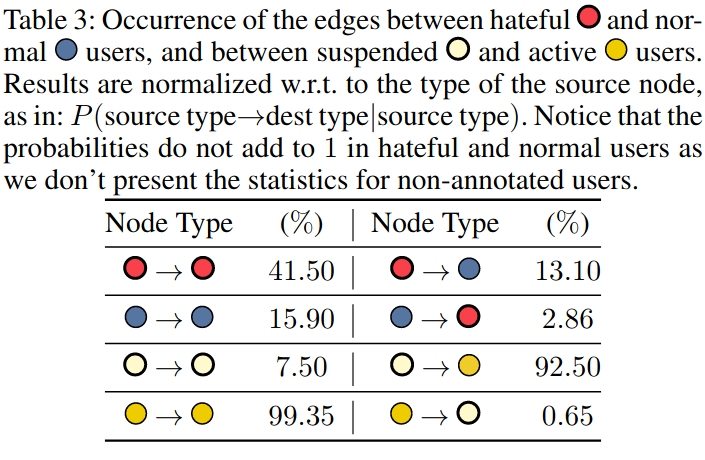
\includegraphics[width=0.8\linewidth]{figures/hatenet}
	\caption{Probabilità di retweet tra i vari tipi di profili codificati nello studio. Immagine pubblicata nello studio del Ribeiro e colleghi (2018).}
	\label{hatenet}
\end{figure}


\section{Discorsi d'odio e politica}
%https://scholar.google.com/scholar?start=10&q=%22hate+speech%22+%22negative+campaign%22&hl=it&as_sdt=0,5
Risulta rilevante constare come vi siano poche ricerche che mettono in correlazione direttamente l'\textit{hate speech} con il \textit{negative campaing}.

L’unico di cui siamo a conoscenza è uno studio condotto durante le elezioni Statunitensi del 2016 che mette in luce come i commenti d'odio online siano condizionati anche dal tipo di comunicazione politica effettuata dai candidati \citep{yacubov2020}. Nello studio sono stati analizzati 1501 commenti di odio a partire da un campione originario di circa 26milioni  contenuti pubblicati in risposta a post di Donald Trump e Hillary Clinton. L'odio è stato selezionato tramite l'utilizzo del dizionario sull'\textit{hate speech} reso disponibile da Hatebase. Su questo sottoinsieme di commenti è stata poi effettuata anche una valutazione qualitativa dividendoli tra incivili e intolleranti. I commenti propriamente incivili (700) o con argomentazioni incivili (394) risultano molto più presenti di quelli intolleranti (164). Dall'analisi del target di questi attacchi [Fig. \ref{fig:hatetarget}], emerge come i gruppi politici rappresentino il bersaglio principale, seguiti dai singoli politici, mentre gli attacchi alle minoranze sono l'1\% dei commenti analizzati. Questi dati sono in linea con quelli riscontrati nella nostra ricerca, come vedremo più avanti.
La relazione tra i discorsi dei politici e i commenti di odio emerge da un'ulteriore analisi qualitativa dei contenuti. Viene riscontrato come gli utenti tendano a riprendere il linguaggio utilizzato dai politici, come ad esempio nel caso della frase “grab her by the pussy”, utilizzata dal presidente in carica durante la campagna e spesso riutilizzata dai suoi sostenitori nei commenti ai suoi post per attaccare altri utenti.
\begin{figure}
	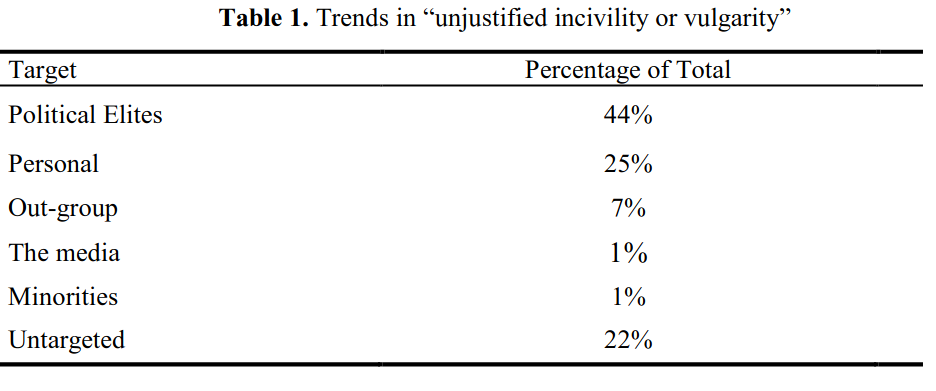
\includegraphics[width=\textwidth]{figures/hatetarget}
	\caption{percentuali dei target a cui sono stati indirizzati gli attacchi incivili e volgari. Immagine pubblicata nello studio di Yacubov (2020).}
	\label{fig:hatetarget}
\end{figure}


%\section{Haters gonna hate}
%-----Although  the  production of hate speech increased dramatically in the wake of all these events, statis-tical models showed it was least likely to be retweeted in volume and to survive for long periods of time, supporting a ‘half-life’ hypothesis. Where hate speech was retweeted, it  emanated  from  a  core  group  of  like-minded  individuals  who  seek  out  each  other’s  messages (Williams and Burnap, 2016)


%da yacubov2020 -->
%studies find that uncivil discourse is a per-vasive  feature  of  online  political  talk,  and  it  is  facilitated  by  several affordances of computer-mediated  communication,  such  as  anonymity  and  the  possibility  to  engage with unknown others, as well as greater likelihood to be exposed to disagreeable per-spectives [2, 3]
%2 Papacharissi,  Z.:  Democracy  online:  civility,  politeness,  and  the  democratic  potential  of online political discussion groups. New Media  Society. 6, 259–283 (2004).


%---> \citep{mondal2017}the effect of anonymity on hate speech and the most hated groups across regions. In order to achieve our objectives, we gather traces from two social media systems: Whisper and Twitter



%ARTICOLI INUTILI:
% 1) i network sono fatti male e parla solo di hastags   --> Network Analysis of “Make America Great Again” di Sean M. Eddington -->  https://journals.sagepub.com/doi/abs/10.1177/2056305118790763
% 2) come gestire le interazion online a livello di intergruppi, ma non parla di hate speech ---> Intergroup contact through online comments: Effects of direct and extended contact on outgroup attitudes --> https://www.sciencedirect.com/science/article/abs/pii/S0747563217306507
% 3) articolo su metoo su twitter, non parla nello specifico di hate speech ma solo di odio https://onlinelibrary.wiley.com/doi/abs/10.1002/poi3.212?casa_token=Ijh0erTEq60AAAAA%3A0a3ChATvWWiqz8iZgah-s-E8b8bzfZLZpYorRh2yKO1MuTlrq0eZy1hE_o2EOSzad7nng-vikPQvzw

%da williams2019 -->
%----Home  Office  (2018)  data  show  that  1,605  hate  crimes  were  flagged  as  online offences between 2017 and 2018, representing 2 per cent of all hate offences. This  represents  a  40  per  cent  increase  compared  to  the  previous  year.  Online  race  hate crime makes up the majority of all online hate offences (52 per cent), followed by sexual orientation (20 per cent), disability (13 per cent), religion (12 per cent) and own  Prosecution  Service  data  show  that in the year April 2017/18, there were 435 prosecutions related to online hate, a 13 per cent increase on the previous year (CPS, 2018)


%ARTICOLI CHE NON CI STANNO PER TEMPO:
% 1) studio sull'odio nei commenti di YT https://www.nomos-elibrary.de/10.5771/2192-4007-2020-1-62/gendered-hate-speech-in-youtube-and-younow-comments-results-of-two-content-analyses-volume-9-2020-issue-1
% 2) odio cyberbullismo e giovani, da qui sono stati presi molti articoli per la biblio, ma non parla di cose del tutto pertinenti https://link.springer.com/chapter/10.1007/978-3-319



